\documentclass[xcolor=dvipsnames]{beamer} 
\usecolortheme[named=BurntOrange]{structure}
\usetheme{shadow} 
\useoutertheme{infolines}
\usepackage{epstopdf}

\author{KACST}
\institute{}
\title{ModExp 4096 Project}
\date{April 2013}

\begin{document}

\begin{frame}
\begin{center}
\textbf{\Large ModExp 4096 \\[0.5em]
Definitions \& Algorithms}  \\[2em]
\c{C}etin Kaya Ko\c{c}  \\
\url{koc@cs.ucsb.edu} \\[3em]
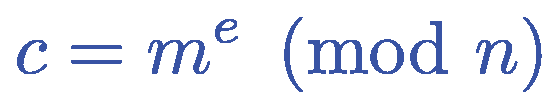
\includegraphics[width=4cm]{cme.eps}
\end{center}
\end{frame}

\begin{frame}{ModExp 4096}
\begin{itemize}

\item These slides describe the architecture, input and output definitions, and
algorithms, and analysis of a 4096-bit full ModExp code

\item The 4096-bit numbers are organized as $sw$ bits, where $s$ is the number
of words and $w$ is the word length, such that $sw=4096$

\medskip

\item We will take $s=128$ and $w=32$ bits in this implementation

\item Additionally the exponent length $k$ is available, as $k \leq 4096$

\end{itemize}
\end{frame}

\begin{frame}{ModExp 4096 Inputs and Output}
\begin{itemize}

\item The \textbf{primary} input parameters are the basis $m$ and the exponent $e$, 
each of which are $s$-word ($sw$-bits: 4096 bits) integers

\medskip

\item The \textbf{secondary} input parameters are $n$, $n0'$, $r$ and $t$, such that
$n$ is the $s$-word ($sw$-bit: 4096-bit) modulus, $n0'$ is a $1$-word ($w$-bit) 
integer, while $r$ and $t$ are $s$-word ($sw$-bit: 4096-bit) integers

\medskip

\item The output $c$ is a $s$-word ($sw$-bit: 4096-bit) integer

\end{itemize}
\end{frame}

\begin{frame}{Primary Input Parameter: $m$}
\begin{itemize}

\item The code assumes that $m$ is a 4096-bit \textbf{signed} integer:
\[
m=(m_{4095}m_{4094}\cdots m_2m_1m_0)
\]
such that $m_{4095}=0$ for $m>0$ due to 2s-complement representation,
and organized as a $s$-word by $w$-bit number: $sw=4096$
\item The LSB is on the top right and
the MSB (the sign bit) is on the bottom left corner, for example,
for $s=4$ and $w=6$, we have

\centerline{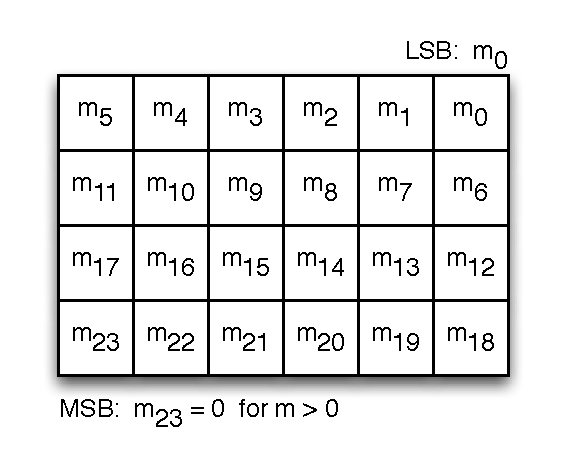
\includegraphics[width=5cm]{m24.eps}}

\item If $m>0$ then $m_{23}=0$; LSB: $m_0$ and MSB: $m_{23}$ (sign bit)

\end{itemize}
\end{frame}

\begin{frame}{Primary Input Parameter: $e$}
\begin{itemize}

\item The exponent $e$ is k-bit \textbf{unsigned} binary number for $k \leq 4096$
\[
e=(e_{k-1}e_{k-2}\cdots e_2e_1e_0)
\]

\item Many practical exponents are fewer than 4096 bits;
we assume $e$ is $k$ bits for $k\leq 4096$

\item The LSB is on the top right and
the MSB (the sign bit) is on the bottom left corner, for example,
for $s=4$ and $w=6$, we have

\centerline{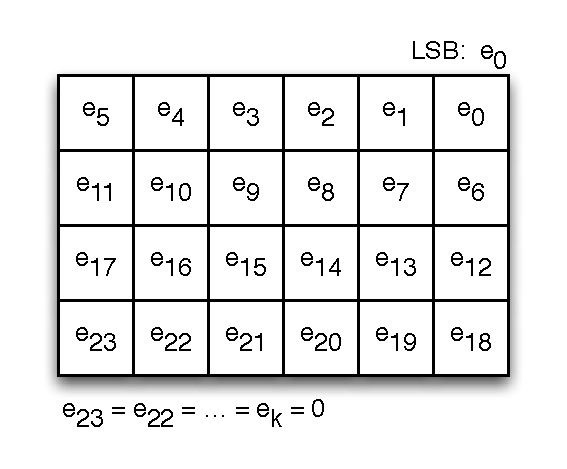
\includegraphics[width=5cm]{e24.eps}}

\item The MSBs $e_{23},e_{22},\ldots,e_k$ are zero

\end{itemize}
\end{frame}

\begin{frame}{Secondary Input Parameter: $n$}
\begin{itemize}

\item The code assumes that $n$ is a 4096-bit \textbf{signed} binary number:
\[
n=(n_{4095}n_{4094}\cdots n_2n_1n_0)
\]
such that $n_{4095}=0$ for $n>0$ due to 2s-complement representation
\item We always have $n_{4095}=0$ ($n>0$) and $n_0=1$ (odd modulus)

\item The LSB is on the top right and
the MSB (the sign bit) is on the bottom left corner, for example,
for $s=4$ and $w=6$, we have

\centerline{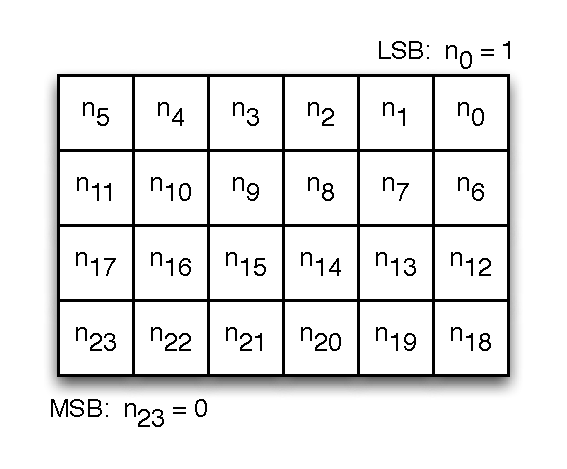
\includegraphics[width=5cm]{n24.eps}}

\item Note that $n_{23}=0$ and $n_0=1$

\end{itemize}
\end{frame}

\begin{frame}{Secondary Input Parameters: $n0'$, $r$ and $t$}
\begin{itemize}

\item The parameters $n0'$, $r$ and $t$ are derived from the modulus $n$:
\begin{eqnarray*}
n0' & = & -n^{-1} \pmod{2^w} \\
r   & = & 2^{sw} \pmod{n} \\
t   & = & 2^{2sw} \pmod{n}
\end{eqnarray*}

\item Since it is often the case that the modulus is fixed, these parameters
are computed at once and saved in the memory
\item The ModExp code assumes that these parameters are available at the
same time with the modulus $n$
\item We will later give code for computing these parameters 
outside the ModExp code

\end{itemize}
\end{frame}

\begin{frame}{Secondary Input Parameters: $n0'$, $r$ and $t$}
\begin{itemize}

\item $n0'$ is a 1-word ($w$-bit) unsigned integer: $n0'=(u_{w-1}\ldots u_1u_0)$
\item $r$ and $t$ are $s$-word ($sw$-bit: 4096-bit) signed integers 

\centerline{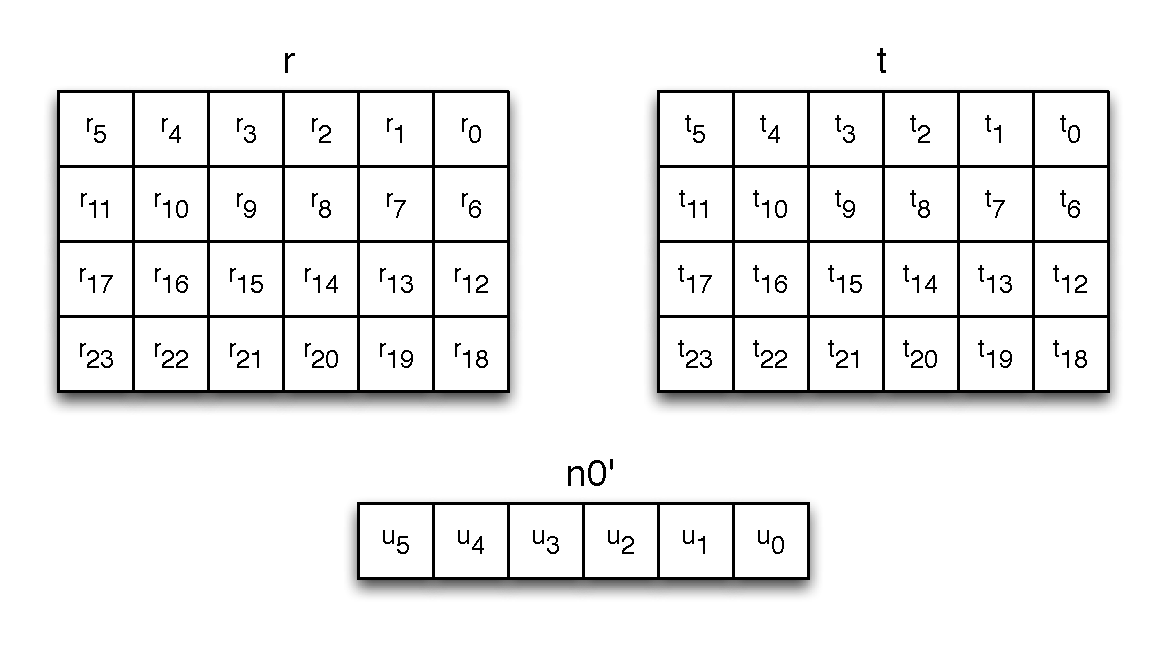
\includegraphics[width=10cm]{secondary.eps}}

\end{itemize}
\end{frame}

\begin{frame}{Target Device \& Properties}
\begin{itemize}

\item The target device is Altera Cyclone II EP2C50
\item This device has 129 $4k$ memory blocks
\item Each $4k$ block can be addressed at different configurations:
$4k\times 1$, $2k\times 2$, up to $128 \times 32$
\item The memory supports byte writes with port data width of
$1,2,4,8,16,32,36$ bits

\item The device has more than sufficient memory of the input and output 
data, as well as for temporary values
\item This allow us to implement several different optimizations on 
the exponentiation level: 1-bit, 2-bit and 4-bit window sizes

\item Some configuration decisions will be made after the coding of the
MonPro block is completed

\end{itemize}
\end{frame}

\begin{frame}{Input and Output}
\begin{itemize}

\item The device assumes the primary inputs $m$ and $e$ are
written into selected memory blocks (GREEN)
\item The device also assumes the secondary input values $n$, $n0'$,
$r$, and $t$ are already written into selected memory blocks (BLUE)
\item It is often the case that the primary values will change after
each computation, while the secondary values will remain in place
\item The device computes $c$ and writes into a memory block (RED)

\centerline{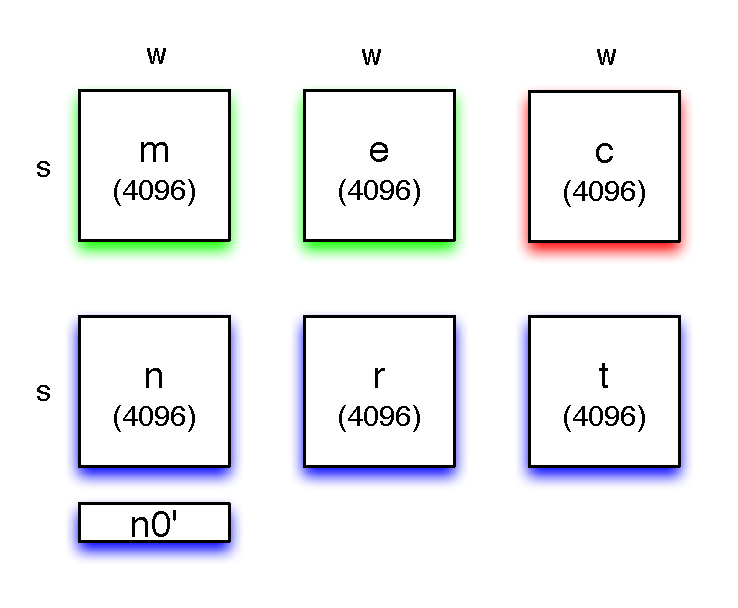
\includegraphics[width=5cm]{io.eps}}
  
\end{itemize}
\end{frame}

\begin{frame}{The ModExp Algorithm}
\begin{itemize}

\item The algorithm of choice is the Montgomery-transformed 
exponentiation using $s$-word integers with a word size of $w$ bits
and the Montgomery constant as $r=2^{sw}$

\item We will describe the 1-bit (binary) and 2-bit (quaternary) 
exponentiation, however, we are experimenting with the 4-bit (hex)
method, and make our final choice at the last phase of the project

\item At the multiplication level, we are using the MonPro CIOS algorithm,
whose details are given later on

\item Primary Inputs: $m$ and $e$
\item Secondary Inputs: $n$, $n0'$, $r$, and $t$
\item Output: $c$
\item Functions: MonPro

\end{itemize}
\end{frame}

\begin{frame}{The $1$-bit ModExp Algorithm}

\hspace*{2em} Find the index $k<4095$ of the leftmost $1$ in $e$ \\
\hspace*{2em} $\bar{m}=\mbox{MonPro}(m,t)$ \\
\hspace*{2em} $\bar{c}=r$ \\
\hspace*{2em} for $i=k-1$ down to $0$ \\
\hspace*{2em} \hspace*{2em} $\bar{c}=\mbox{MonPro}(\bar{c},\bar{c})$ \\
\hspace*{2em} \hspace*{2em} if $e_i=1$ then $\bar{c}=\mbox{MonPro}(\bar{c},\bar{m})$ \\
\hspace*{2em} $c=\mbox{MonPro}(\bar{c},1)$

\end{frame}

\begin{frame}{The $2$-bit ModExp Algorithm}

\hspace*{2em} Express $e$ in 2-bit blocks $e=(E_{2047}\cdots E_1E_0)$ with
$E_j \in \{0,1,2,3\}$ \\
\hspace*{2em} Find the index $k<2047$ of the leftmost nonzero in $e$ \\
\hspace*{2em} $\bar{m}1=\mbox{MonPro}(m,t)$ \\
\hspace*{2em} $\bar{m}2=\mbox{MonPro}(\bar{m}1,\bar{m}1)$ \\
\hspace*{2em} $\bar{m}3=\mbox{MonPro}(\bar{m}2,\bar{m}1)$ \\
\hspace*{2em} $\bar{c}=\mbox{MonPro}(1,t)$ \\
\hspace*{2em} for $i=k$ down to $0$ \\
\hspace*{2em} \hspace*{2em} $\bar{c}=\mbox{MonPro}(\bar{c},\bar{c})$ \\
\hspace*{2em} \hspace*{2em} $\bar{c}=\mbox{MonPro}(\bar{c},\bar{c})$ \\
\hspace*{2em} \hspace*{2em} if $E_i=1$ then $\bar{c}=\mbox{MonPro}(\bar{c},\bar{m}1)$ \\
\hspace*{2em} \hspace*{3em} else if $E_i=2$ then $\bar{c}=\mbox{MonPro}(\bar{c},\bar{m}2)$ \\
\hspace*{2em} \hspace*{4em} else if $E_i=3$ then $\bar{c}=\mbox{MonPro}(\bar{c},\bar{m}3)$ \\
\hspace*{2em} $c=\mbox{MonPro}(\bar{c},1)$

\end{frame}

\begin{frame}{The MonPro Algorithm}
\begin{itemize}

\item The MonPro algorithm takes two inputs: $x$ and $y$,
and computes the output $z$ such that each variable 
holds an $s$-word ($sw$-bit: 4096-bit) signed integer:
$x=(x_{s-1}x_{s-2}\cdots x_1x_0)$,
$y=(y_{s-1}y_{s-2}\cdots y_1y_0)$, and 
$z=(z_{s-1}z_{s-2}\cdots z_1z_0)$ with $x_i,y_i,z_i$ as $w$-bit
for $s-1 \geq i \geq 0$, and the initial value of $z$ is zero

\item The secondary inputs $n$, $n0'$, $r$ and $t$ are also available;
we particularly need $n0'$ and $n$, which are $1$-word and $s$-word integers

\centerline{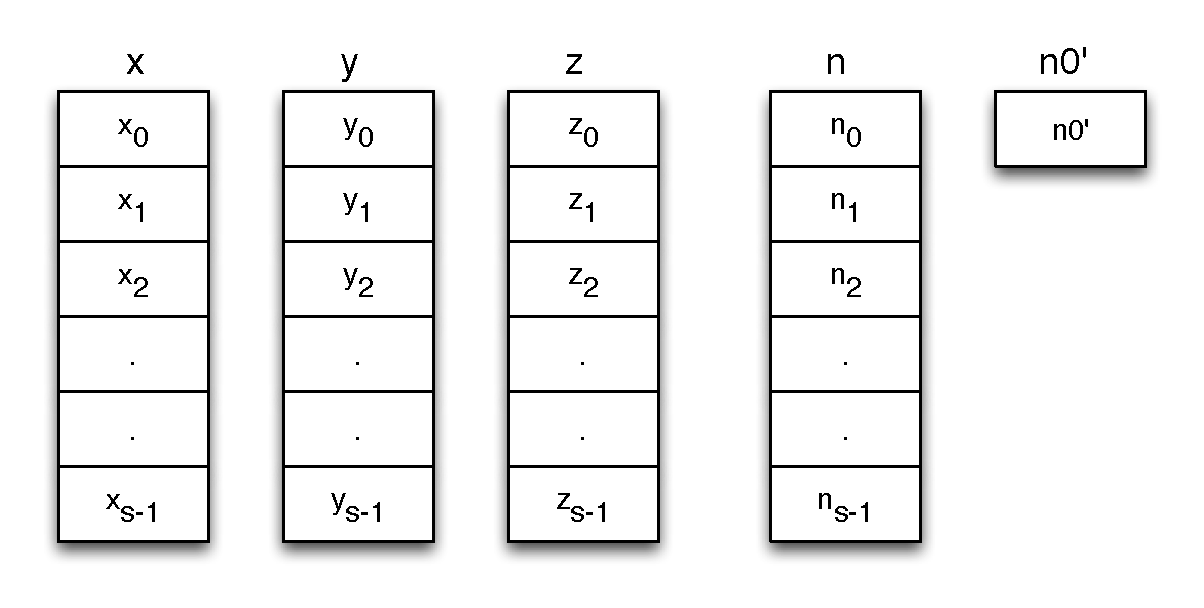
\includegraphics[width=7cm]{mp0.eps}}

\end{itemize}
\end{frame}

\begin{frame}{The MonPro Algorithm}
\begin{enumerate}

\item[1:] We take the LSW of $x$, namely $x_0$ and multiply by the $s$-word $y$,
and add it to the $s$-word partial product $z$ (which is now all zero) to  obtain
the $(s+1)$-word temporary result $v$ as
\[
v = x_0 \cdot \sum_{i=0}^{s-1} y_i 2^{wi} + \sum_{i=0}^{s-1} z_i 2^{wi}
\]

\centerline{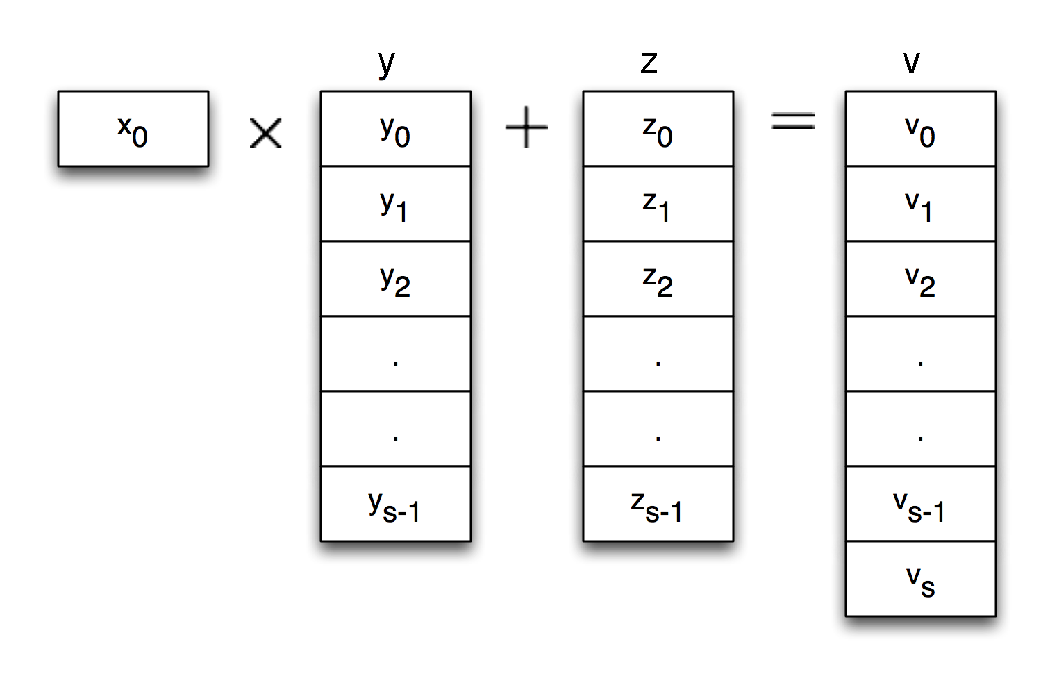
\includegraphics[width=7cm]{mp1.eps}}

\end{enumerate}
\end{frame}

\begin{frame}{The MonPro Algorithm}
\begin{enumerate}

\item[1a:] The computation in Step 1 is accomplished using a Multiply-Add block
that multiplies two 1-word numbers ($x_0$ and $y_0$), adds the previous higher word ($C_0$), and adds another 1-word number ($z_0$), producing a 2-word number ($C_1,S_0$); the lower word word ($S_0$) is assigned to ($v_0$), while the higher word ($C_1$) is kept
for the next Multiply-Add step, as follows:
\begin{eqnarray*}
(C_1,S_0) & = & x_0 \cdot y_0 + C_0 + z_0 \\ 
v_0 & = & S_0 \\
(C_2,S_1) & = & x_0 \cdot y_1 + C_1 + z_1  \\
v_1 & = & S_1 \\
(C_3,S_2) & = & x_0 \cdot y_2 + C_2 + z_2 \\
v_2 & = & S_2 \\
& \cdots &
\end{eqnarray*}
such that the initial value $C_0=0$

\end{enumerate}
\end{frame}

\begin{frame}{The MonPro Algorithm}
\begin{enumerate}

\item[2:] Then, we take the LSW of $v$, namely $v_0$ an multiply by the $1$-word
$n0'$ modulo $2^{w}$ and obtain the $1$-word integer $m$ as
\[
m = n0' \cdot v_0 \pmod{2^w}
\]

\centerline{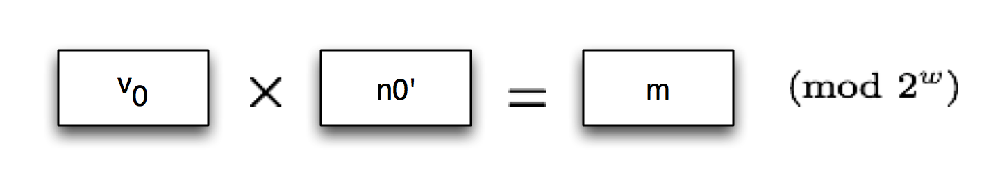
\includegraphics[width=8cm]{mp2.eps}}

\end{enumerate}
\end{frame}

\begin{frame}{The MonPro Algorithm}
\begin{enumerate}

\item[3:] Then, we take the $1$-word $m$ and multiply by the $s$-word $n$,
and add it to the $(s+1)$-word temporary value $v$ to obtain the new
partial product which is $(s+1)$-word
\[
z = m \cdot \sum_{i=0}^{s-1} n_i 2^{wi} + \sum_{i=0}^{s} v_i 2^{wi}
\]

\centerline{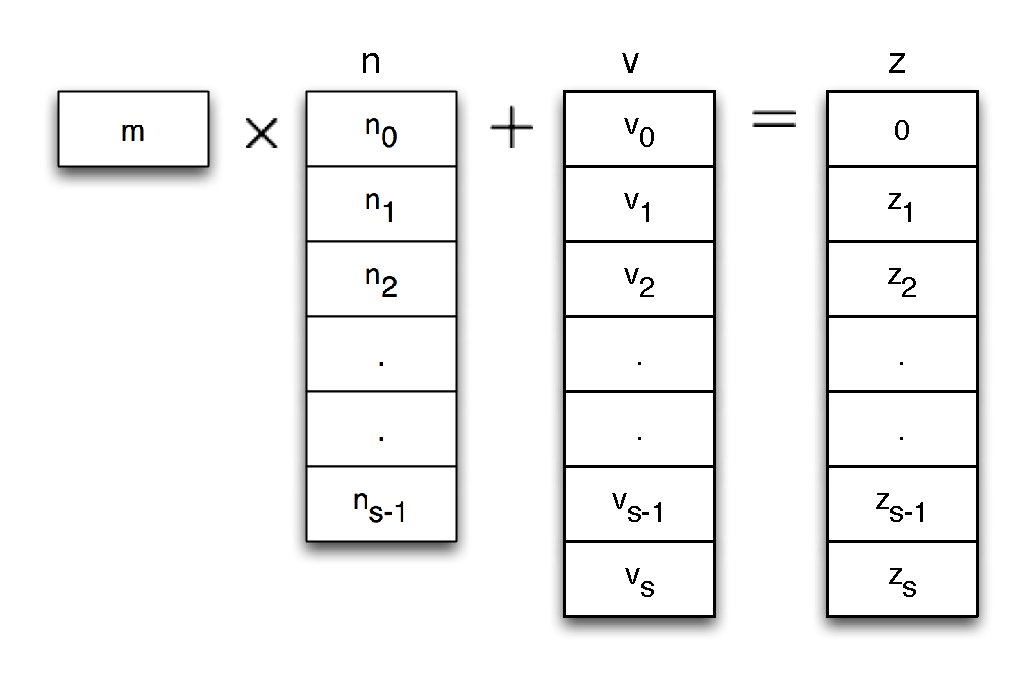
\includegraphics[width=6cm]{mp3.eps}}

\end{enumerate}
\end{frame}

\begin{frame}{The MonPro Algorithm}
\begin{enumerate}

\item[3a:] The computation in Step 3 is accomplished using a Multiply-Add block
that multiplies two 1-word numbers ($m$ and $n_0$), adds the previous higher word($C_0$), adds another 1-word number ($v_0$), producing 
a 2-word number ($C_1,S_0$); assigning $S_0$ to $z_0$, while keeping the higher word ($C_1$)
for the next Multiply-Add step, as follows:
\begin{eqnarray*}
(C_1,S_0) & = & m \cdot n_0 + C_0 + v_0\\
z_0 & = & S_0 \\[0.5em]
(C_2,S_1) & = & m \cdot n_1 + C_1 + v_1 \\
z_1 & = & S_1 \\[0.5em]
(C_3,S_2) & = & m \cdot n_2 + C_2 + v_2 \\
z_2 & = & S_2 \\
& \cdots &
\end{eqnarray*}
such that the initial value $C_0=0$

\end{enumerate}
\end{frame}

\begin{frame}{The MonPro Algorithm}
\begin{enumerate}

\item[4:] The resulting partial product $z$ has its LSW as zero, due to
the Montgomery property, and therefore, we shift up $z$ to obtain
the new $s$-word partial product

\centerline{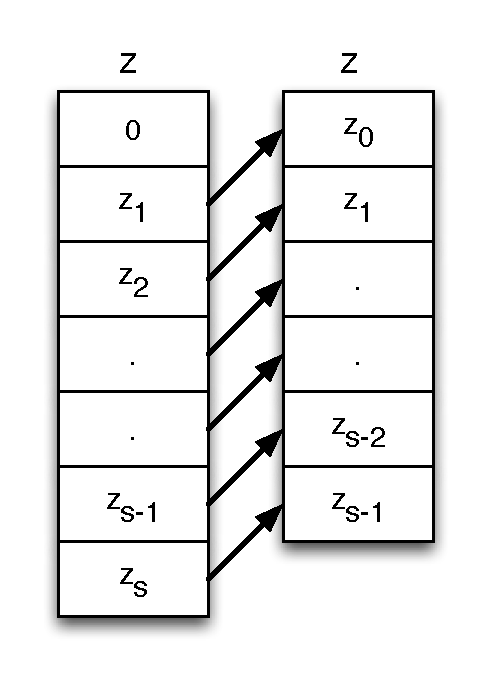
\includegraphics[width=4cm]{mp4.eps}}

\end{enumerate}
\end{frame}

\begin{frame}{The MonPro Algorithm}
\begin{enumerate}

\item[5:] In the next step the next word of $x$, namely $x_1$, is taken and
multiplied with the $s$-word $y$, and added to the partial
product $z$ to obtain the new temporary result $v$ as
\[
v = x_1 \cdot \sum_{i=0}^{s-1} y_i 2^{wi} + \sum_{i=0}^{s-1} z_i 2^{wi}
\]

\centerline{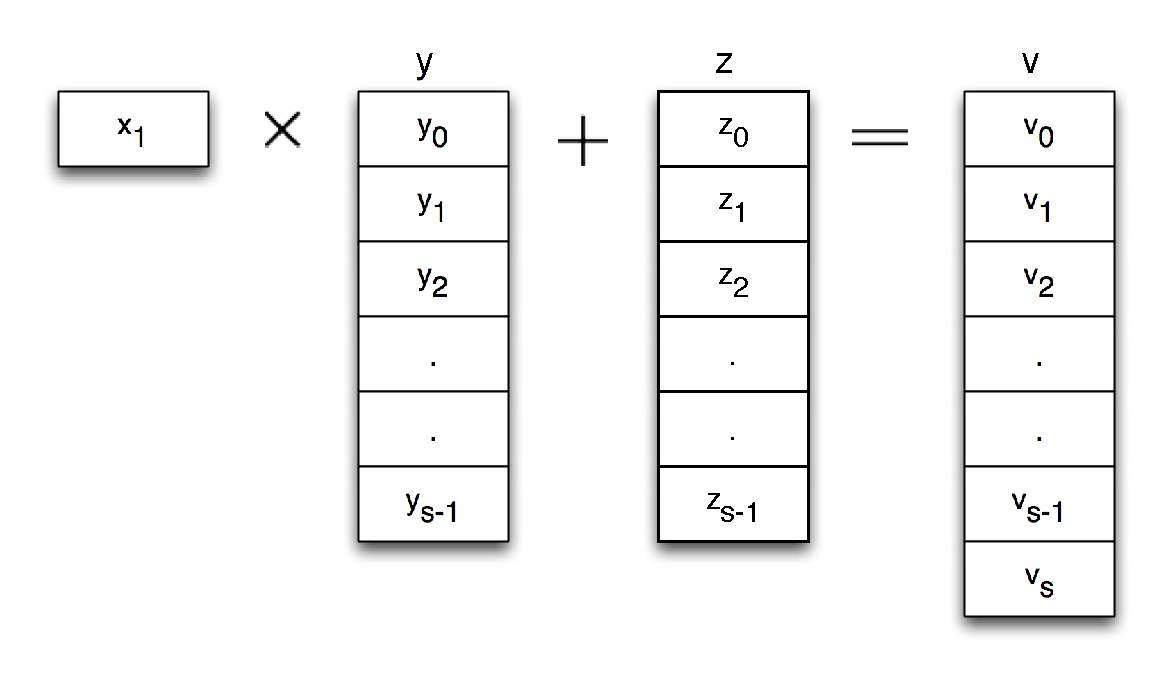
\includegraphics[width=7cm]{mp5.eps}}

\end{enumerate}
\end{frame}

\begin{frame}{The MonPro Algorithm}
\begin{enumerate}

\item[6:] This is followed up by computing the new $m$ value
\[
m = n0' \cdot v_0 \pmod{2^w}
\]
and then the multiplication of $m$ by $n$, and then the addition of the
result to $v$ to obtain the new $(s+1)$-word partial product $z$
\[
z = m \cdot \sum_{i=0}^{s-1} n_i 2^{wi} + \sum_{i=0}^{s} v_i 2^{wi}
\]
and finally shifting up $z$ by one word (since $z_0=0$) to obtain
the new $s$-word $z$ value

\item[7:] Proceeding in this way, we multiply all $x_i$ values by the
multiplicand $y$ and reduce it modulo $n$, for $i=0,1,2,\ldots, s-1$

\end{enumerate}
\end{frame}

\begin{frame}{Resources and Components}
\begin{itemize}

\item The ModExp requires implementation of several blocks
\item A finite state machine to scan the bits of the exponent, 1-bit, 2-bit
and 4-bit at a time
\item A $w$-by-$w$ bit integer multiplier producing $2w$-bit products
\item A $w$-by-$w$ bit integer adder producing $(w+1)$-bit sums
\item A finite state machine to control the flow of the MonPro algorithm
from $i=0$ to $i=s-1$

\item Several registers for the primary and secondary inputs, for the output,
and for the temporary values

\end{itemize}
\end{frame}

\begin{frame}{Interface}
\begin{itemize}

\item Our analysis shows that $w=32$ and $s=128$ values will produce an
implementation that will satisfy the specified requirements

\item The target device Altera Cyclone II EP2C50 has 129 $4k$ memory
blocks which can be configured as $128 \times 32$

\item At this configuration these memory blocks are not accessible 
in the true dual-port mode, however, we will not need that

\item It is therefore assumed that the initiating processor uploads
the $128$-word primary inputs $m$ and $e$, and $128$-word secondary 
inputs $n$, $r$, and $t$, and $1$-word secondary input $n0'$ to 
selected memory blocks

\item The ModExp code will run and produce the $128$-word output $c$
in a selected memory block

\end{itemize}
\end{frame}

\begin{frame}{Interface}
\begin{itemize}

\item The ModExp code will not destroy the input values and all of them can
be reused for subsequent executions

\item It is generally the case the primary inputs $m$ and $e$ will be
refreshed by the initiating processor, leaving the secondary input
values $n$, $r$, and $t$, and $n0'$ intact for subsequent execution(s)

\end{itemize}
\end{frame}

\end{document}
